
\documentclass[sigconf]{acmart}

%%
%% \BibTeX command to typeset BibTeX logo in the docs
\AtBeginDocument{%
  \providecommand\BibTeX{{%
    \normalfont B\kern-0.5em{\scshape i\kern-0.25em b}\kern-0.8em\TeX}}}

%% Rights management information.  This information is sent to you
%% when you complete the rights form.  These commands have SAMPLE
%% values in them; it is your responsibility as an author to replace
%% the commands and values with those provided to you when you
%% complete the rights form.
\setcopyright{acmcopyright}
\copyrightyear{2019}
\acmYear{2019}
\acmDOI{}

%% These commands are for a PROCEEDINGS abstract or paper.
%\acmConference[Woodstock '18]{Woodstock '18: ACM Symposium on Neural
%  Gaze Detection}{June 03--05, 2018}{Woodstock, NY}
%\acmBooktitle{Woodstock '18: ACM Symposium on Neural Gaze Detection,
%  June 03--05, 2018, Woodstock, NY}
%\acmPrice{15.00}
%\acmISBN{978-1-4503-9999-9/18/06}

\begin{document}

\title{Re-Comparison of Two Proactive Self-adaptation Methods: PLA and CobRA}

\author{Ben Trovato}
\authornote{Both authors contributed equally to this research.}
\email{trovato@corporation.com}
\orcid{1234-5678-9012}
\author{G.K.M. Tobin}
\authornotemark[1]
\email{webmaster@marysville-ohio.com}
\affiliation{%
  \institution{Institute for Clarity in Documentation}
  \streetaddress{P.O. Box 1212}
  \city{Dublin}
  \state{Ohio}
  \postcode{43017-6221}
}

\author{}
\affiliation{%
  \institution{The Th{\o}rv{\"a}ld Group}
  \streetaddress{1 Th{\o}rv{\"a}ld Circle}
  \city{Hekla}
  \country{Iceland}}
\email{larst@affiliation.org}

\author{}
\affiliation{%
  \institution{Inria Paris-Rocquencourt}
  \city{Rocquencourt}
  \country{France}
}
%\begin{verbatim}
%\bibliographystyle{ACM-Reference-Format}
%\bibliography{acmart}
%\end{verbatim}

\begin{abstract}
Software-intensive systems face the challenge of uncertainties at runtime which need the ability to adapt itself to keep satisfying the requirements. Recently, there are two proactive approaches, namely PLA and Cobra, which implement the self-adaptation from the perspective of software engineering and control theory respectively and both of them adopt the ideas from model predictive control (MPC). In order to provide a guidance to select an approach, Gabriel et al. have compared the two approaches in aspects of development cost, run-time performance and the efforts to achieve desired adaptation effects. They claimed that both of them can achieve the similar satisfying adaptation results. In this paper, we revisit their comparison of the two approaches by exploring the principle for similar adapatations and further investigating their differences and superiorities in case of environment prediction, asymmetric latency and actuation regularizer. We apply the two appraoches to the benchmark system called RUBiS as Gabriel et al. do and reuse their self-adaptation scenario. It is shown that the environment prediction mechanism of PLA contributes less to a better self-adaptation comparing to the implicit feedback mechanism. Moreover, CobRA doesn't model asymmetrical latency which may get poor adaptation results.
\end{abstract}

\begin{CCSXML}
	<ccs2012>
	<concept>
	<concept_id>10011007.10010940.10010971</concept_id>
	<concept_desc>Software and its engineering~Software system structures</concept_desc>
	<concept_significance>300</concept_significance>
	</concept>
	</ccs2012>
\end{CCSXML}

\ccsdesc[300]{Software and its engineering~Software system structures}
\keywords{self-adaptation, PLA, CobRA, model predictive control}
\maketitle

\section{Introduction}
Software-intensive systems suffer uncertainties at runtime, such as fluctuant running environment, changing requirements and unexpected operating conditions which often reduce the quality of service delivery~\cite{filieri2015software}. Therefore, self-adaptation is required to eliminate or mitigate the adverse effects of uncertainties. Software self-adaptation is the ability to adapt to uncertainties for continously delivering high-quality services through the dynamic reconfiguration of its parameters or architecture~\cite{calinescu2017engineering}. A self-adaptive system is often implemented as MAPE-K loop~\cite{kephart2003vision} which consists monitor, analyze, plan, and execute modules sharing a whole knowledge, shown in Figure ~\ref{fig:mape}. For each loop, the monitor module calculates statistical values of the measurements captured by sensors and then the analyze module and plan module, together referred to as descision-making module, generates an adaptation strategy, often corresponding to a set of adaptation tactics, such as adding a server, and finally the execute module will deploy these tactics by effectors. 

\begin{figure}[h]	
	\centering	
	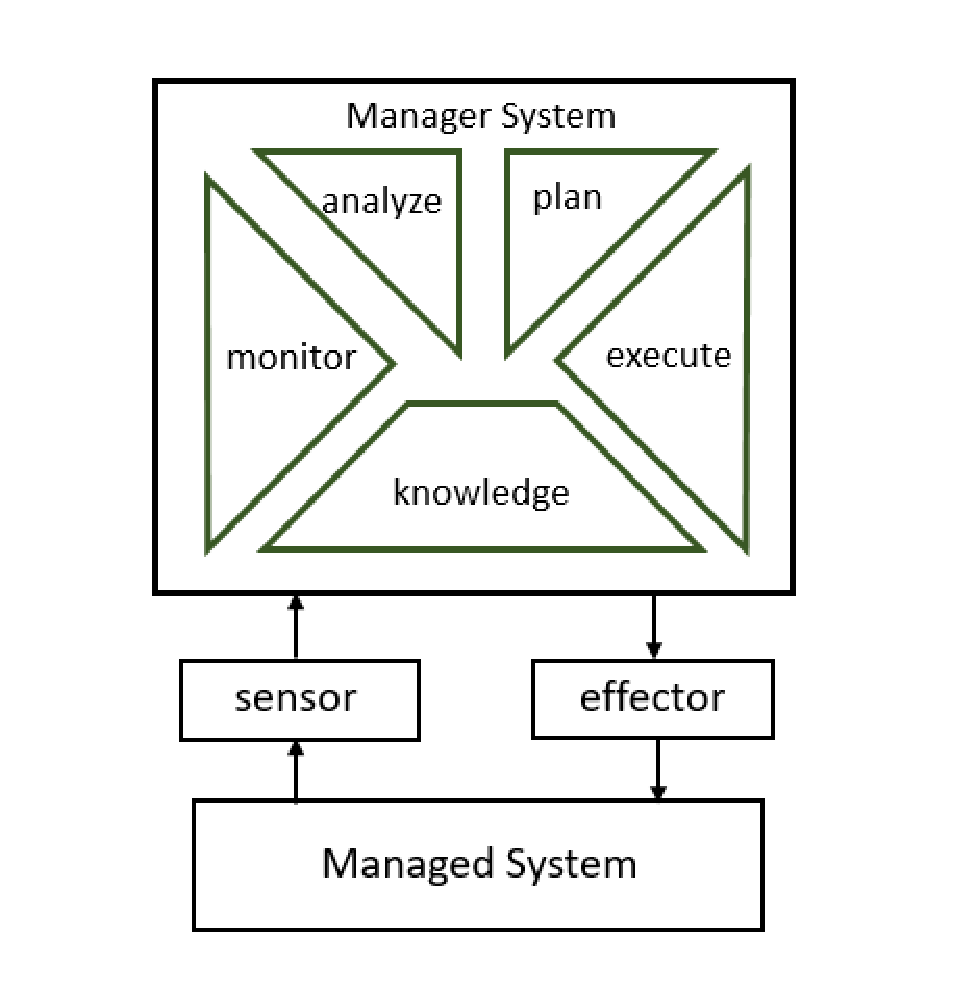
\includegraphics[width=\linewidth]{mape}	
	\caption{MAPE-K architecture}	
	\label{fig:mape}	
\end{figure}

The early approaches of software self-adaptation are reactive, namely they calculate adaptation tactics only based on the captured changes but do not consider changes in the future and the effects of adaptation tactics are regarded to be instant. Correspondingly, the later proposed proactive self-adaptation approaches predict future changes to make an adaptation strategy ahead of time and can handle tactic latency between when the tactic is deployed and when the effect is shown.

In the control field, model predictive control (MPC)~\cite{qin2003survey} regards the controlled system as a black-box, often modelled as a linear system, with multiple inputs and outputs. It uses the current measurments, the predicted future outputs for a receding horizon based on system model and the known constrainsts to generate the desired inputs for the receding horizon. To implement software self-adaptation, two main proactive approaches, PLA~\cite{moreno2015proactive} and CobRA~\cite{angelopoulos2016model}, are proposed. Both of them adopt the ideas from MPC, but have different implementations. Both of them use prediction models to predict future behavior of the managed software system, but PLA describes the possible future behavoir of software system inculding tactic latency and its environment as an integrated Markov decision process (MDP) and tries to predict the future changes of the environment based on historical measurements while CobRA is aimed at introduce model predictive control directly based on specific assumptions. Cobra regards the system as a linear model and treats the changing environment as disturbance. Moreover, Both of them adopt the idea of receding horizon which calculates a sequence of adapation strategies for each loop but only selects the first one. 

Despite of the different implementations, the two proactive self-adaptation approaches are all proven to be effective. When we are considering to implement a proactive self-adaptive system, which one should we choose? Gabriel et al. have compared the two approaches in the light of development costs and run-time performance and shown their similar adaptation effects on a benchmark~\cite{moreno2017comparing}. But they did not analyse why PLA and Cobra can achieve the similar adapation effect and investigate the capabilities of their different implementations for handling uncertainties. 

Therefore, based on their work, we try to give an explanations for similar adapatation effects, such as the constraints of model parameters and enumerate the different implementations of the two approaches for handling uncertainties and further analyze their advantages and disadvantages, providing a detailed guidance for approach selecting. We analyzed the differences between the two from three aspects, including 1) modeling environment, 2) asymmetric latency and 3) regular terms for optimization. We theoretically analyzed the reasons and effects of the differences, and follow the same experiment senarios of ~\cite{moreno2017comparing} to verify our conjecture.

In the remainder of the paper, Section II presents the adaptation scenario we used. Section III provides an overview of CobRA and PLA both on design and implementation. Next, Section IV gives an explanations for their similarities. Section V describes three different aspects of CobRA and PLA. Finally, Section VI presents our conclusions and the future work.

\section{adaptation senario}
The same as~\cite{moreno2017comparing}, we carry out our comparison on the RUBiS system~\cite{ow22013rubis}, an open-source auction site prototype modeled after eBay.com which is widely used for evaluating self-adaptation and cloud computing~\cite{qin2003survey,islam2015online}. As shown in Figure~\ref{fig:rubis}, RUBiS consists of a load-balancer, a web server tier and a database tier. Clients use browsers to send requests to the system. Load balancer distributes requests among servers following a round-robin policy. Then, servers access the database to obtain the data to render the page which includes mandatory content and optional content. Providing optional content such as recommendations of similar auction items for users can achieve more revenue but need more response time and an intolerable response time may lead to high penalty. Therefore, a brownout RUBiS~\cite{klein2014brownout} is proposed which gradually downgrade the possibility of optional content for user requests, called dimmer, for handling high workload. In order to keep and reproduce the same experimental conditions for the two approaches, we run our experiments on a simulated system of brownout RUBiS, called SWIM.

\begin{figure}[!htp]
	\centering
	
\includegraphics[width=\linewidth]{rubis}
	\caption{Architecture of RUBiS}
	\label{fig:rubis}
\end{figure}

The self-adapation goal of RUBiS is to capture the maximum revenue of user requests with the minimum server cost in spite of the uncertainties. There are three non-functional requirements concerned with our self-adaptation goal: the first one is keeping the response time $r$ below the threshold $T$; the second one is the target system shall provide high quality of content, namely maximize dimmer $d$; the third one is that the target system shall operate under low cost, namely minimize the number of servers $s$. Then, the adaptation goal can be formally expressed as a utility function of these three requirements as follows:

\begin{equation}
\begin{aligned}
U_{\tau}=\left\{
\begin{array}{rcl}
U_{R}+U_{C} & & { r\leq T\wedge U_{R}=U_{R}^{*}} \\
U_{R} & & {r\leq T\wedge U_{R}<U_{R}^{*}}\\
\tau min(0,\alpha-\kappa)R_{O} & & {r>T}\\
\end{array} \right.
\end{aligned}
\end{equation}
	
\noindent$U_{C}$ represents the utility associated with \textit{cost} per time interval:
	
\begin{equation}
\begin{aligned}
U_{C}=\tau \cdot c\cdot (s^{*}-s)
\end{aligned}
\end{equation}

\noindent and $U_{R}$ represents the utility associated with revenue per time interval:
\begin{equation}
\begin{aligned}
U_{R}=\tau \cdot \alpha \cdot (d\cdot R_{O}+(1-d)\cdot R_{M})
\end{aligned}
\end{equation}

\noindent where $\tau$ is the length of the interval, $\alpha$ is the average request rate, and \textit{d} is dimmer value. $R_{M}$ and $R_{O}$ are the rewards for serving a request with mandatory and optional content respectively. We have $R_{O}>R_{M}>0$.

For RUBiS, there are two known kinds of uncertianties, namely 1) arrival rate of user requests and 2) latency of booting a server which can be measured aftertime and it provides two types of tactics to adjust itself to deal with these uncertainties:
\begin{itemize}
	\item {\verb|Add/remove a server|}:
	The two tactics are used to change the number of servers $s$. There is a delay in adding a server whereas the delay of removing a server can be ignored.
	
	\item  {\verb|Increase/decrease dimmer value|}:
	The two tactics are used to change the value of dimmer $d$ which indicates the proportion of a request including optional content ($d\in[0,1]$) and the effect of them are regarded to be instant. 
\end{itemize}

\section{Two proactive self-adaptaion methods: PLA and CobRA}
Both PLA and CobRA adopt the ideas of model predcitive control (MPC) to implement software self-adaptation but use different ways. Next, we will describe PLA and CobRA in terms of design details and implementations.

\subsection{PLA}
PLA uses DTMCs to model the probabilistic behavior of the environment and the managed system including tactic delay, leave adaptation decision underspecified through nondeterminism and then use the probabilistic model checker to find the nondeterministic choices that maximize the accumulated utility over the horizon~\cite{moreno2015proactive}. 

For each adaptation period $\tau$, PLA uses an autoregresive (AR) time series predictor, such as RPS toolkit~\cite{dinda2006design}, to predict the distribution of each environment variable and applies the Extended Pearson-Tukey (EP-T)~\cite{keefer1994certainty} three point approximation to construct probability trees for next environment prediction. As shown in Figure~\ref{fig:envtree}, the root $e_{0}$ is the current value of a environment variable $e$ and $e_{i}$ is the next $i$th predicted distribution of this environment variable. The three point values are the 5th, 50th and 95th percentiles of the predicted distribution with transition probabilities 0.185, 0.630 and 0.185 respectively. It should be noted that there are often large deviations between the predicted values of the environment and the real ones because it is hard to satisfy the assumption that the changes of environment should be predictable. 

\begin{figure}[!htp]
	\centering	
	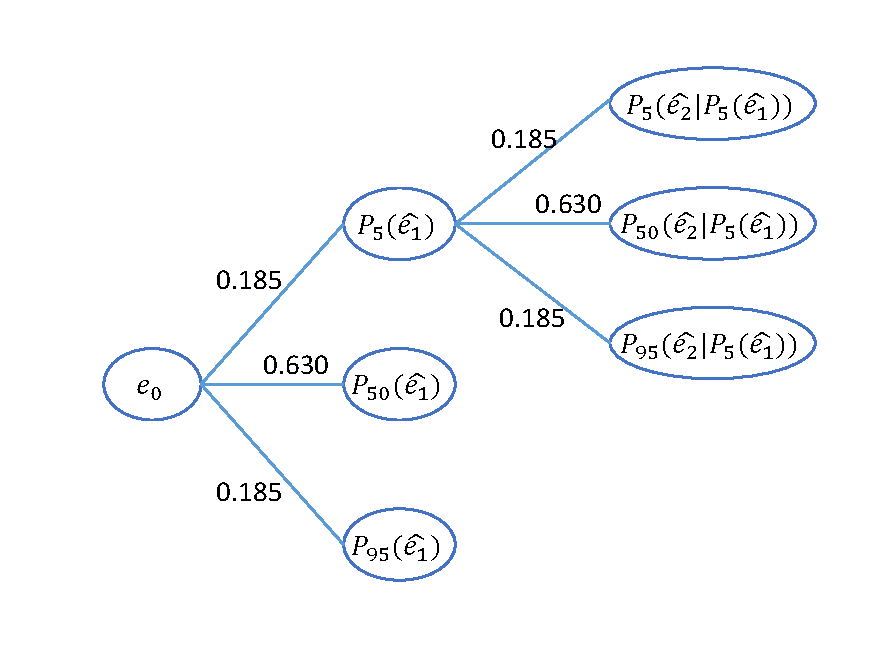
\includegraphics[width=\linewidth]{envtree}	
	\caption{Probability Tree of Environment}
	\label{fig:envtree}
\end{figure}

The managed system accompanied with adaptation tactics is modeled as a Markov decision process (MDP)~\cite{puterman2014markov} which uses state transitions to express all possible execution of adaptation tactics for handling the environment predictions. We can use a probabilistic model checker~\cite{moreno2015proactive}, such as PRISM~\cite{kwiatkowska2011prism} to exhaust state transitions of adaptation tactics over the horizon and find a path of state transitions (a strategy) to maximize the accumulated value of the utility function defined above. PLA accurately models the relationship between measurable requirement-related variables and adaptation parameters. For example, It uses LPS queuing theory model~\cite{zhang2008steady} to calculate the response time under specified configurations of server and dimmer. Obviously, the adaptation performance of PLA is highly relied on the prediction values, thus it needs plenty of effort to build an accurate model of the environment and the target system in design time.

\subsection{CobRA}
CobRA implements the self-adaptive system directly from control theory and the adaptation decision is aimed to find the right balance (equilibrium) between the conflicting requirements by maximizing the utility-based cost funtion defined as:

\begin{equation}
\begin{aligned}
&J_{k}=\sum_{i=1}^H [y_{k+i}^o -\hat{y}_{k+i}]^TQ_{i}[y_{k+i}^o -\hat{y}_{k+i}] \\
&+[\Delta u_{k+i-1}]^T P_{i}[\Delta u_{k+i-1}]
\end{aligned}
\end{equation}

where $y$ represents the set of measurable requirement-related variables called \textit{indicators} and $u$ represents a set of adaptation parameters called \textit{control parameters}. $y_{k+i}^o$ and $\hat{y}_{k+i}$ are setpoints (goals) and predicted values of indicators at next $i$-th adaptation period respectively. $Q_{i}$ and $P_{i}$ are symmetric positive semi-definite wetghting matrics. $Q_i$ means that when not all the goals can be achieved, the controller will prefer the satisfaction of the goals with high weights. $P_i$ means that the controller want to change the control parameters frequently with smaller weight. For RUBiS system, the indictors is the average response time \textit{r} for user requests and the \textit{control parameters} are the number of servers \textit{s} and the dimmer value \textit{d}. As same to PLA, The control interval of CobRA is $\tau$ and at the start of each interval, a sequence values of control parameters over the horizon are calculating by controller.

CobRA abstracts the relationship between indictors and control parameters as a simple discrete-time linear model as follows:

\begin{equation}
\left\{
\begin{array}{rcl}
x(k+1)=A\cdot x(k)+B\cdot u(k)\\
y(k)=C\cdot x(k)+D\cdot a(k)\\
\end{array} \right.
\end{equation}

\noindent where $x$ is the set of system states which is often a immeasurable variables but links control parameters to indicators ~\cite{maggio2017automated} and $a$ represents measurable environment variables, such as arrival rate of user requests, which cannot be tuned can be used as a feedforward signal and $k$ represents the k-th adaptation loop. Unlike PLA, CobRA does not predict the changes of future environment but treats the changes of environment as disturbance to the system instead. In our scenario, the known uncertianty of environment is arrival rate of user requests.

Above all, the self-adaptation decision of CobRA is to solve the optimization problem at start of each period definited as follows:

\begin{equation}
\begin{aligned}
&minimize_{\Delta u_{k+i-1}}\qquad J_t \\
&subject\quad to \qquad u_{min}\leq u_{k+i-1}\leq u_{max},\\
&{\Delta u_{min}}\leq{ \Delta u_{k+i-1}}\leq {\Delta u_{max}},\\
&\tilde{x_{k+i}}=\tilde{A}\cdot \tilde{x_{k+i-1}}+\tilde{B}\cdot \Delta u_{k+i-1}, \\
&y_{k+i-1}=\tilde{C}\cdot \tilde{x_{k+i-1}},\\
&\quad i=1,...,H,\\
&x_{k}=x(k)
\end{aligned}
\end{equation}
\noindent where $\Delta u_{min}$ and $\Delta u_{max}$ are the constraints for changing control parameters while $u_{min}$ and $u_{max}$ are the saturation values of control parameters. CobRA makes adaptation decisions to keep indicators as close to their setpoints as possible while satisfying those constraints. 

\section{Similarities}
In the work of G.A\cite{moreno2017comparing}, they show that both of them can handle those uncertainties and maximize the system's utility. We reproduced their experiments and get conclusions even further. We explore the reasons why the two different methods can get similar adaptation control results.

In our experiment, we use the same workload: WorldCup\cite{arlitt2000workload} and ClarkNet\cite{arlitt1996web} as Gabriel et al. did and system parameters and utility functions are follwing the settings in \ref{moreno2015proactive}. 


\begin{figure}[h]
	\centering
	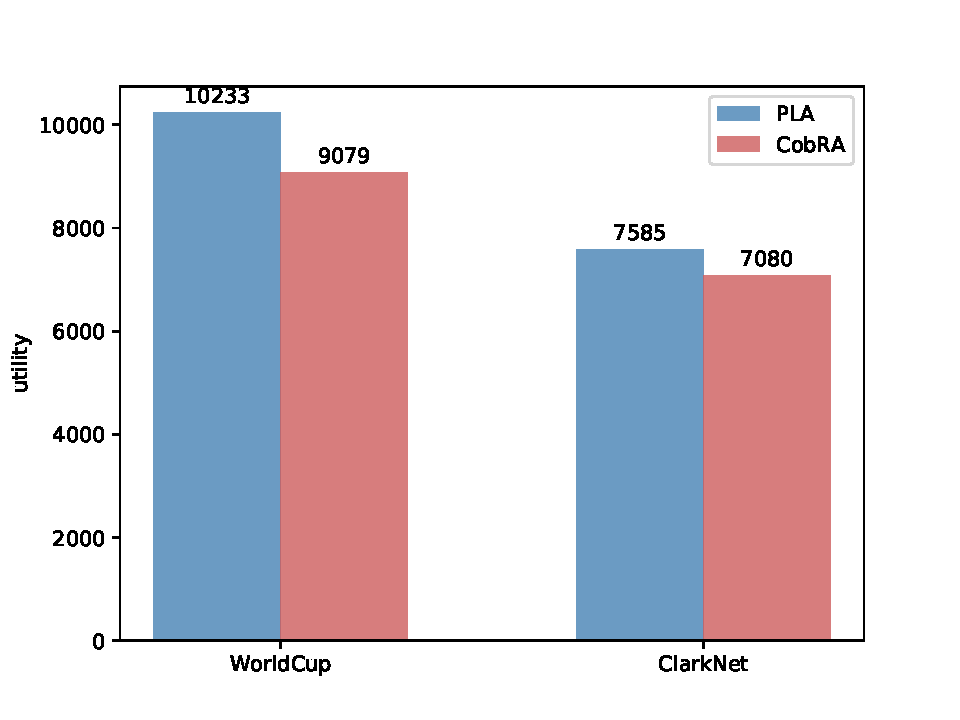
\includegraphics[width=\linewidth]{utility-simi}
	\caption{Results of utility}
	\label{utility-simi}
\end{figure}
\begin{figure*}[h]
	\centering
	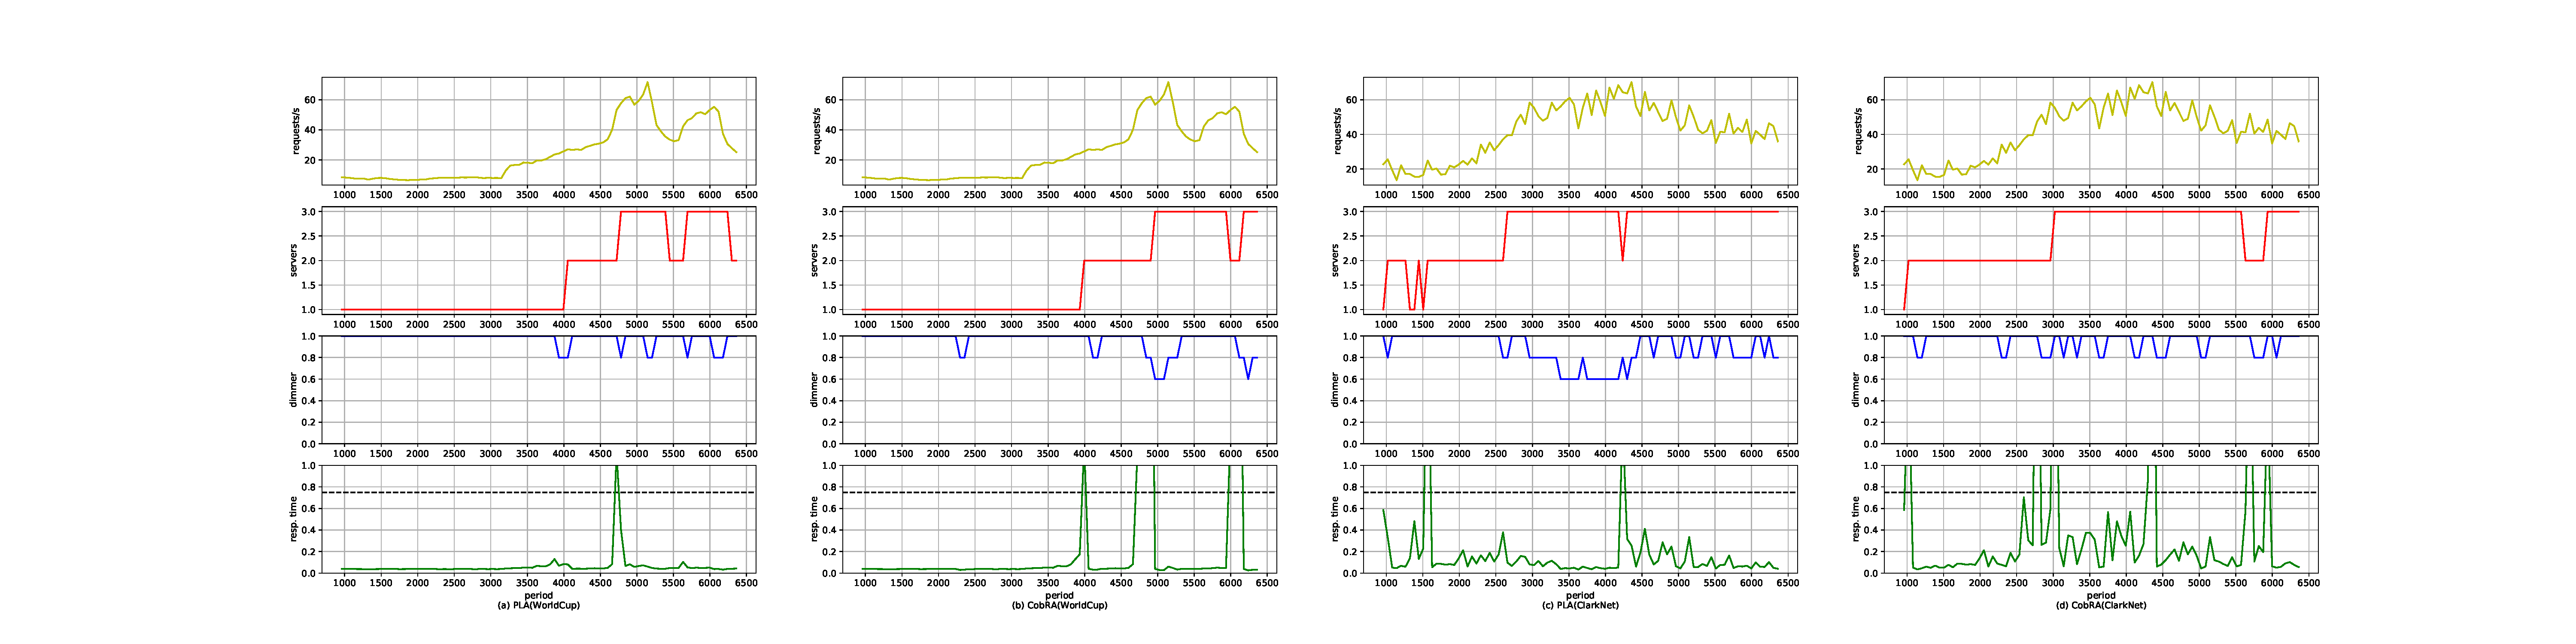
\includegraphics[width=\linewidth]{similarity}
	\caption{Control results of PLA and CobRA}
	\label{similarity}
\end{figure*}

We show total utilities of PLA and CobRA under the two workloads in Figure~\ref{utility-simi} and Figure~\ref{similarity} show the detailed control results of the two methods under the two workloads. We get utility values more than theirs results and compared to CobRA, PLA can achieve better control results. 


\subsection{Feedback in PLA and CobRA}

The reason for this is we find that both of the two methods heavily depend on the strength and rate of feedback. If we can adjust feedback parameters to a favourable value, we an get even better results of self-adaptation.  Through feedback control, PLA can decrease the errors between model and real system to keep $r$  below the threshold as far as possible. However, simple feedback control has some weaknesses resulting in CobRA's slight poor performance than PLA, which we discuss in section IV.

The important factor influencing CobRA's decision making is the setting of parameters in the cost-function and system model, which was also argued in the work of GA. CobRA relies heavily on the value of weight matrix, feedback adjustment parameters and setpoint value, which determine the optimal solution of cost-function.

Although PLA is an open-loop method in terms of architecture, that is, the control effect at current decision period does not affect the decision making at the next period. Open-loop methods can only handle disturbance in measurements and modeling. However, there are many uncertain disturbance in PLA. First, it is inevitable that there will be errors in environment prediction. Second, in implementation, PLA uses LPS queuing model\cite{zhang2008steady} to simulate system's service mode and calculate the average response time of requests. Although LPS model is a pretty accurate description of limited process sharing system with round-roubin strategy, it's calculated value is the indicators when the system gets a steady state. However, when the system's running, it is difficult to achieve stable states as a result of the load fluctuation.
Therefore, there will be errors between the calculated value of queuing model and the actual response time of the system actually. As the system is exponential, when the threshold is triggered, the difference will be significant, which will affect PLA to make correct decisions. However, PLA can still achieve similar effects as CobRA under errors in modeling and prediction because PLA uses feedback in the implementation.
In the work of GA\cite{thesis}, it is proposed that in the process of implementation, Kalman Filter is used to dynamically adjust the value of service rate according to the differences between the calculated value and the real value of response time. In fact, it adjusts the servicetime parameter $st$ of the system, which is the value describing the service capability of the system and should not be adjusted with the change of workload. So this adjustment is just to make the model more realistic, which is not much reasonable.
\begin{figure}[h]
	\centering
	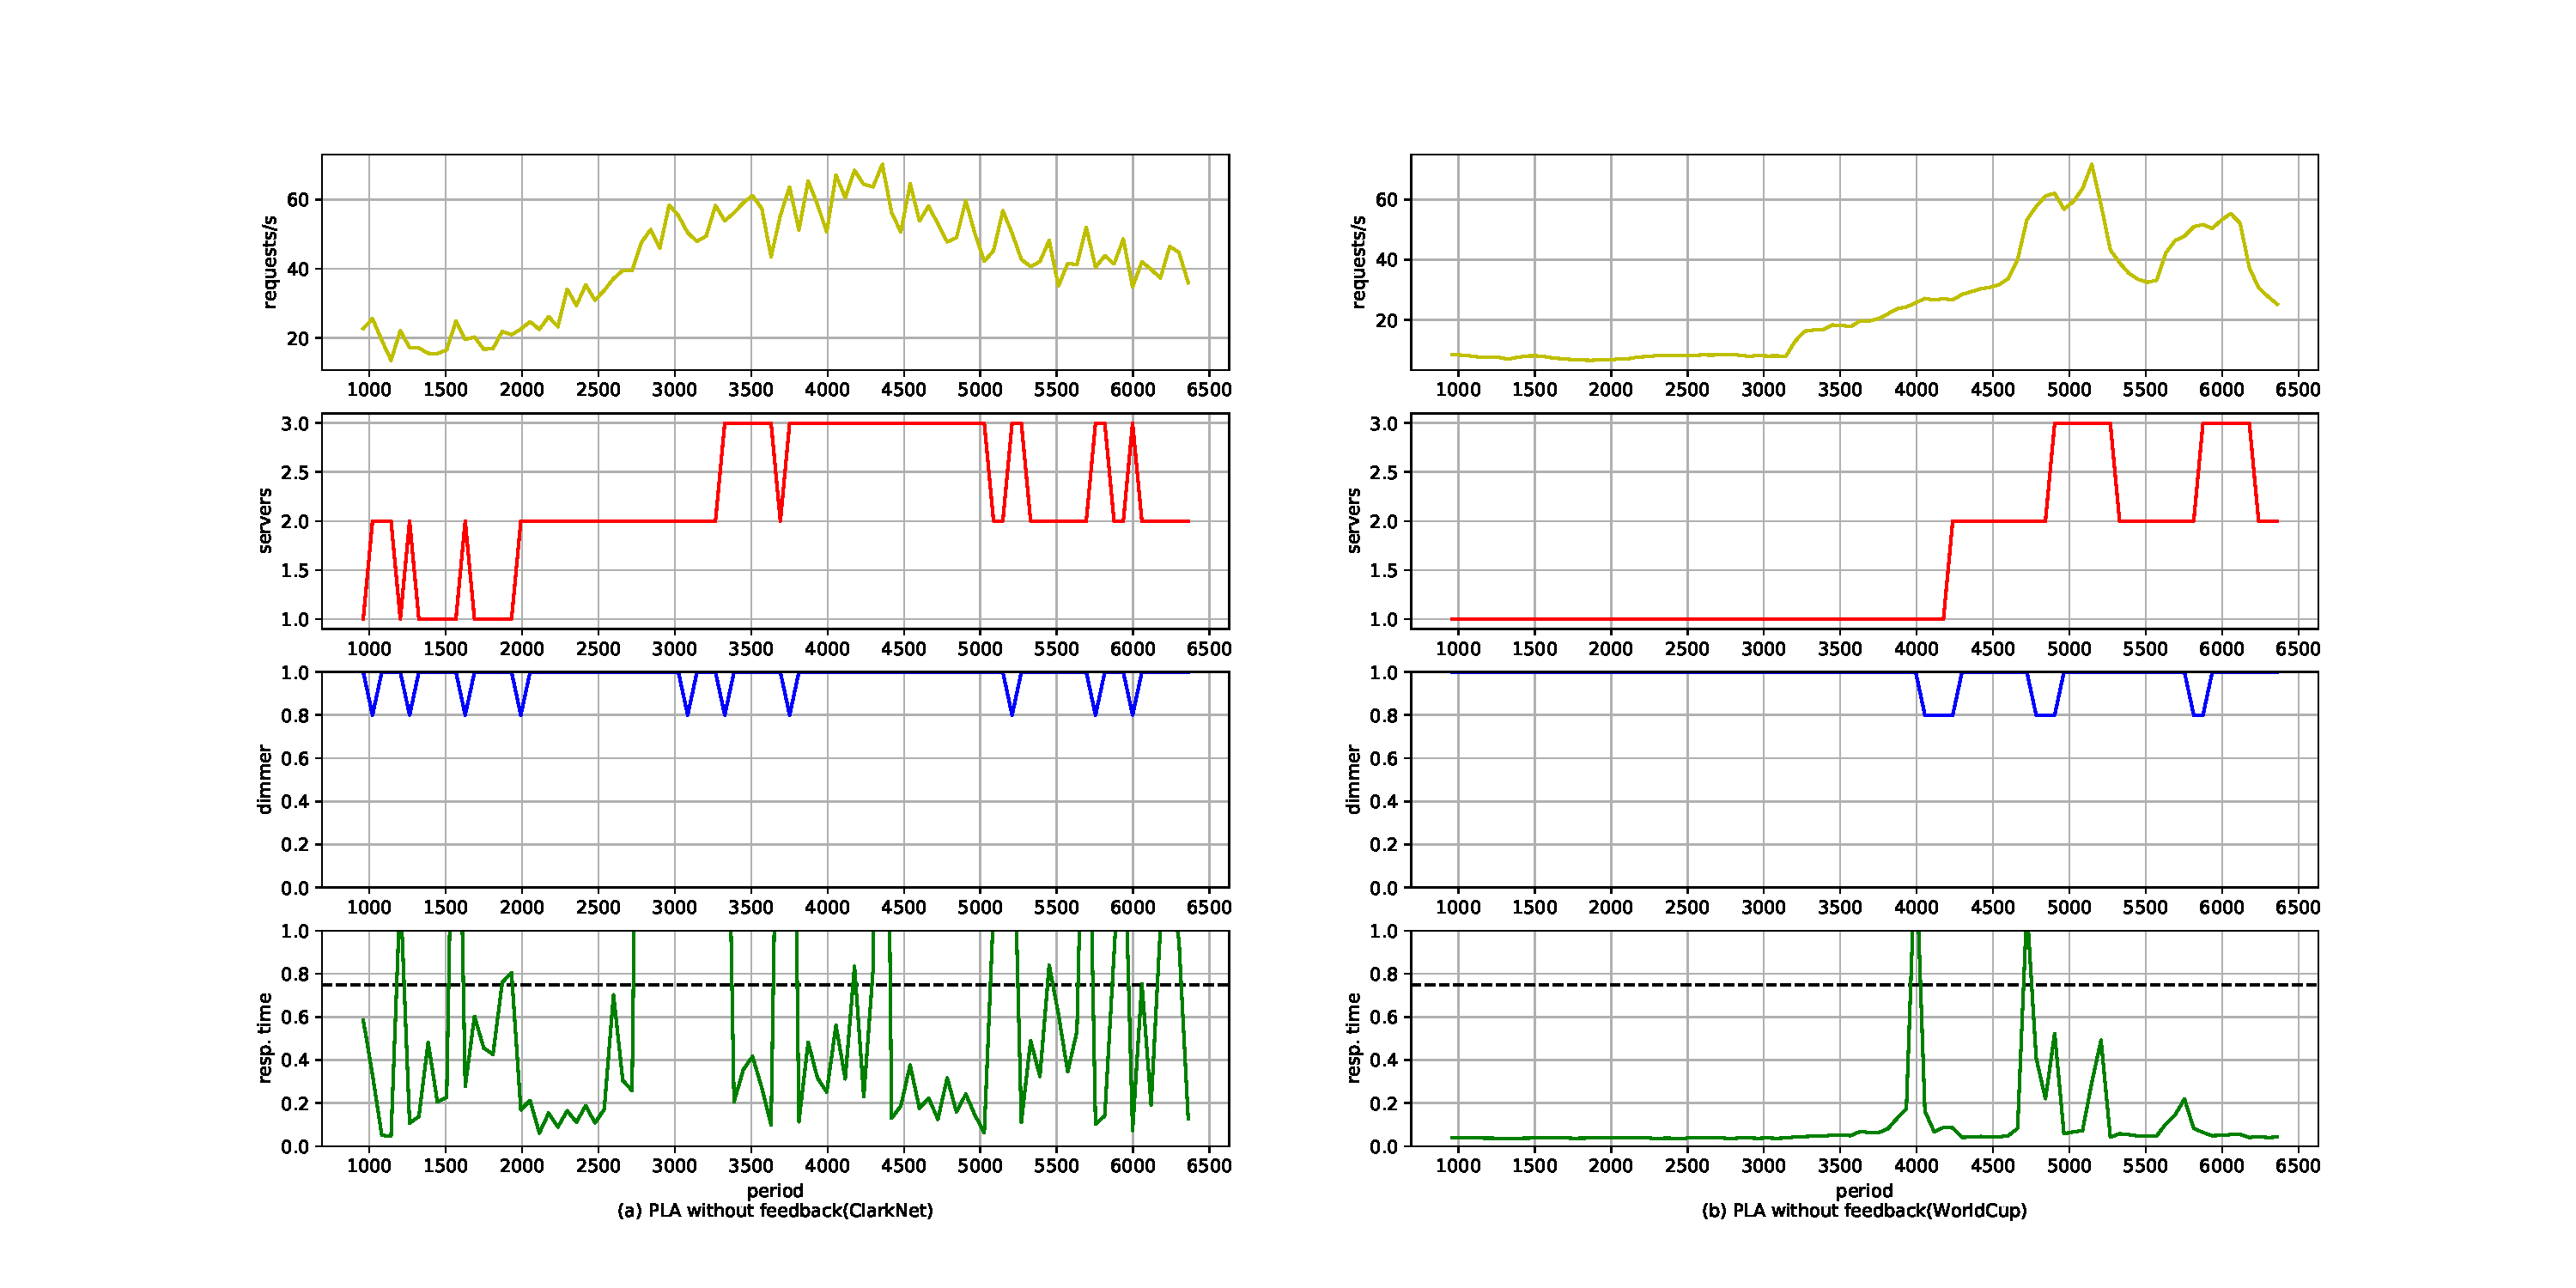
\includegraphics[width=\linewidth]{nokalman}
	\caption{Control effects of nkPLA}
	\label{nokalman}
\end{figure}
\begin{figure}[h]
	\centering
	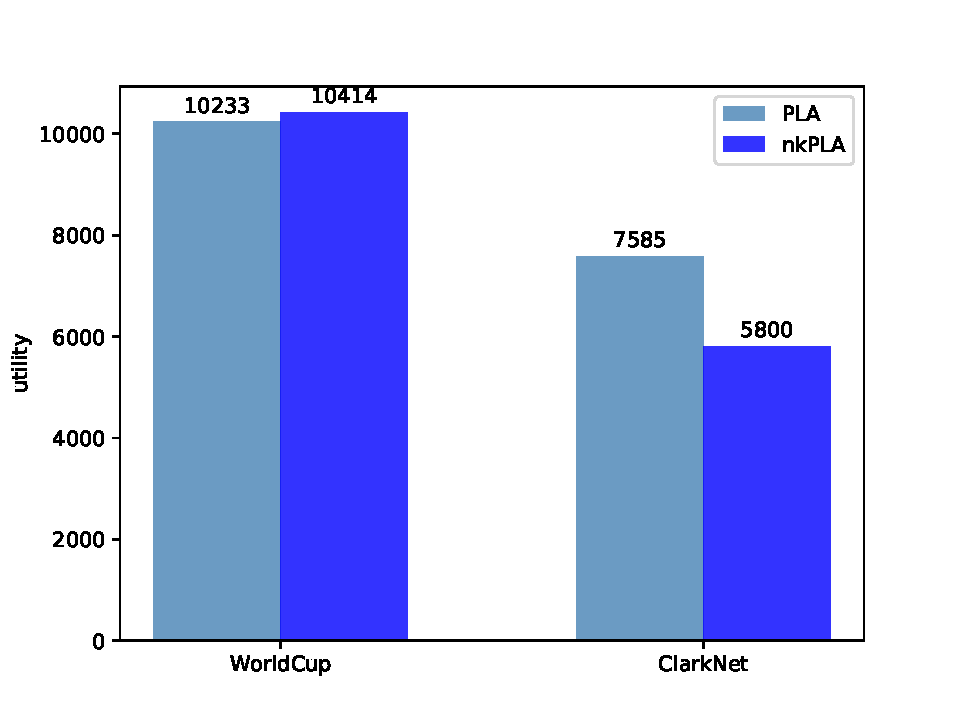
\includegraphics[width=\linewidth]{utility-nk}
	\caption{Comparation of utility between PLA and nkPLA}
	\label{utility-nk}
\end{figure}
To explore the effect of feedback, we construct a variant of PLA, named as nkPLA, which does not use feedback and just depends on prediction. We compare the self-adaptation effects of PLA with nkPLA. Figure~\ref{nokalman} shows the results of no feedback under two workloads and Figure~\ref{utility-nk} compares the utility with PLA. Under the ClarkNet, there are several period the response time exceeding the threshold $T$ but PLA's controller does not make adaptation decisions to handle it. That is because the response time calculated by the queuing theory model is below the threshold value. However, PLA makes decisions based on the calculated value, and it is determined that no control decisions need to be made at this moment. Thus the utility is much lower than with feedback. However, the utility of nkPLA is slightly lower than PLA under WorldCup. That is because the characteristics of this workload and the natural defect of feedback. WorldCup is much stable and then meets a sudden ascend. Although without feedback PLA can't handle the model error, feedback will tend to make tactics conservativly to guarentee the system's stability. Thus the number of servers can not decrease timely, which lead to lower utility value.



\subsection{Adaptation Decision}


The decision-making of these two methods are actually two different constrained optimization problems. We assume that the two methods are excuting in the same situation. Under this precondition, we disscus the reasons why they can achieve similar control effects under so many differences by deducing their adaptation decision process. For convenience of comparison, we express the control action in the form of "augmented velocity form" of control variables $\Delta u$.
%Under the current measured system configuration and environment state, that is, known $s_0$, $d_0$ and $a$, by solving this optimization problem, we can get the control increment, $\Delta s$ and $\Delta d$to minimize $u$ while satisfying their constraints. Because of PLA's prediction for environment, in every decision period in the horizon, $a$ is the prediction of future prediction, which is different from CobRA following.
CobRA's modeling for requirements can be described as a quadratic constrained optimization problem. In control theory, it is most common to use quardratic performance indices to achieve smooth and robust control results. It can be described as:
\begin{equation}
	\begin{aligned}
		&J_k=\sum_{i=1}^{H_p}((y_{k+i}^2-y_{k+i}))^TQ_i(y_{k+i}^2-y_{k+i})\\
		&+(\Delta u_{k+i-1}^T)P_i(\Delta u_{k+i-1}))
	\end{aligned}
\end{equation}
We use $H_p$ to denote the length of prediction horizon and $H_u$ denote the control horizon. The control action $u_{k|k}$ at time $k$ can be get from CobRA's optimization problem.
\begin{equation}
	u_(k|k)=[I_q\quad 0\quad 0\cdots](\theta^T Q\theta+R)^{-1}\theta^T Q(r_k-\psi _(\hat{x}_{k|k})
\end{equation}
where
\begin{equation}
	\begin{aligned}
		&\psi=[(CA)^T (CA^2)^T\cdots(CA^H_p)^T]^T\\
		&\theta=
		\left[
		\begin{matrix}
			CB & 0_{n\times q} &\cdots & 0_{n\times q} \\
			CAB & CB& \cdots   & 0_{n\times q}\\
			\vdots & \quad& \ddots&\vdots\\
			CA^{H_p-1}B& \quad&\cdots&CA^{H_p-H_u-1}B
		\end{matrix}
		\right]\\
		&Q=diag(Q_1,\cdots,Q_{H_p})\\
		&R=diag(R_0,\cdots,R_{H_u-1})\\
		&r_k=[r_{k+1}^T\quad r_{k+2}^T\quad \cdots r_{k+H_p}^T\quad]^T
	\end{aligned}
\end{equation}
and $u_(k|k)$ is the control input applying at time $k$ and is extracted from $u_k$ and is the solution of the optimization problem. $\hat{x}_(k|k)$ denotes the estimated value of state $x_k$ at time $k$. We can get the $\hat{x}_(k|k)$ by using Kalman Filter as follows:
\begin{equation}
	\begin{aligned}
		&\hat{x}_{k|k}=\hat{x}_{k|k-1}+L_k(y_k-C\hat{x}_{k|k-1})\\
		&\hat{x}_{k+1|k}=A\hat{x}_{k|k-1}+K_k(y_k-C\hat{x}_{k|k-1})\\
		&L_k=P_kC^T(CP_K C^T+DD^T)^(-1),K_k=AL_k\\
		&P_{tk+1}=AP_tA^T-K_k(CP_kC^T+DD^T)K_k^T
	\end{aligned}
\end{equation}
For PLA, its modeling for utility can be translated into a linear constrained optimization problem. Maximizing utility in the control horizon at period $k$ can be transformed into minimizing the minus of utility, $u$, which can be expressed as follows:
\begin{equation}
	\begin{aligned}
		&min\quad u_k=\sum_{i=1}^{H_p}((s_{k+i}+\Delta s_{k+i}*cost\\
		&-\dfrac{d_{k+i}+\Delta d_{k+i}}{a_{k+i}}*(R_{O}-R_{M}))), 
	\end{aligned}
\end{equation}
under the circumstance that:
\begin{equation}
	r_k\leq T 
\end{equation}
We use LPS model to calculate the average response time at period k $E[r]_k$ by knowing measured system states:
\begin{equation}
	\begin{aligned}
		&E[r]_k\approx( \dfrac{{c_a}_k^2+{c_s}_k^2}{2}\times \dfrac{\beta_k}{1-\rho_k}\times {d_p}_k\\
		&+\dfrac{{c_a}_k^2+{c_s}_k^2}{1+{c_s}_k^2}\times \dfrac{\beta_k}{1-\rho_k} \times (1-{d_p}_k)) \\
&where\\
&(d_p)_k\approx \rho_k^(\dfrac{1+{c_s}_k^2}{{c_a}_k^2+{c_s}_k^2}K)\\
&\rho_k=\beta_k \times \lambda_k\\
&\beta_k=d_k\times st_k+(1-d_k)\times lst_k\\
&\lambda_k=\dfrac{1}{a_k \times s_k}
\end{aligned}
\end{equation}	
We consider that the environment is an upward trend. The calculated $r$ of CobRA is lower than the real value because CobRA  does not predict the trend of workload. Thus CobRA depends on Kalman Filter to catch the trend of workload and modify the system state. PLA can predict approximate future variation tendency of workload. In addition to prediction errors, queuing theory is apt at modeling systems at steady state. However, during running it is rather difficult for the system to get steady state. Workload fluctuates will lead to requests's backup in servers and result in the inconsistency between prediction and measurement. Therefore, Kalman Filter modify the $st$ dynamically according to the distance between calculated and measured $r$, the same as CobRA. Turn up $st$ reults in higher calculated $r$ in next period.

Compared to simple proportional control which does not use receding horizon to predict future system but just use a certain proportion to reflect errors, proactive self-adaptations such as PLA and CobRA can deal with system tactics that have latency in launch. Because if the controller does not consider future state, when the workload is increasing and needs more servers to provide satisfying service, the controller can not predict to add a server ahead of time to deal with the latency.

We can get the conclusion that when there are inevitable errors in prediction and model, the way for PLA to solve these uncertainties is to use feedback. PLA can achieve satisfying control results under so much errors heavily depends on feedback, the same as CobRA.

We can get the conclusion that, the reasons that PLA and CobRA can get similar control result have two aspects: 
\begin{itemize}
	\item {\verb|Adopt ideas and structures of MPC.|}:
	First, both of them use models to predict future system behavior, but the models of them are different. Second, both of the employ receding horizon to make the adaptation decision robust and accurate. In addition, 
	\item {\verb|Heavily depend on feedback|}:
	They both use feedback to decrease errors between model and the real system, and to reduce the impact from disturbance. Although from the perspective of architecture, PLA is an open-loop method. It needs feedback to deal with errors in prediction for environment and system behavior.	
\end{itemize}

\section{Differences}
While PLA and CobRA can achieve similar adaptation effect, there are some differences between them, which are mainly described in table~\ref{tab:differences}. We mainly investigate four significant differences, namely 1) environment handling; 2) system modeling; 3) asymmetric tactic delay handling and 4) constraints of regular terms and explore how these differences affect the adaptation decisions of PLA and CobRA.

\begin{table*}
	\caption{Differences between PLA and CobRA}
	\label{tab:differences}
	\begin{tabular}{ccl}
		%\newcommand{\tabincell}[2]{\begin{tabular}{@{}#1@{}}#2\end{tabular}}
		\toprule
		Features&PLA&CobRA\\
		\midrule
		Method & Architecture-based& Requirement-based\\
		Model for Environment & DTMC model
		& Feedforward signal 
		\\
		Feedback & Open-loop
		& Closed-loop\\
		Control  & tactics& Control parameter values
		\\
		Discrete or Continuous&Discrete&Continuous\\
		Unsymmetric Latency&Model the unsymmetric latency&Can not model the unsymmetric latency
		\\
		Total Model&Non-linear MDP Model&Linear Dynamic Model\\
		Optimization&Utility function&System goals following boolean AND/OR semantics\\
		
		\bottomrule
	\end{tabular}
\end{table*}

\subsection{Environment Handling}
While implementing the self-adaptation of managed software system, PLA and CobRA handle the changes of environment differently. PLA assumes the changing envrionment is predicatale and uses current and historical measurements to construct the probabilistc tree of future environment. Then, the predicted environment will be used to calculate the accumulated utility for all possible adaptation strategies and the adaptation strategy corresponding to maximum accumulated utility is our adaptation decision. Whereas CobRA regards the assumed slowly changing environment as disturbances which is handled by closed-loop feedback control. Thus, it does not predict future environment but uses its measurements as a feedforward signal to improve the prediction of current indicators which is used for Kalman Filter to obtain the true states of current system. 

When the environment changes regularly and easy to predict accurately, decision-making with future environment prediction is theoretically better than no prediction like CobRA beacause the effect of future envrionment changes on managed system can be considered ahead of time. However, the accurate environment prediction is hard to obtained and there is often deviation of system model. Practically, PLA uses feedback mechanism to handle model deviation. In this section, we want to explore the effect of PLA's environment prediction on adaptation decision-making. 

We design a variant of PLA, denoted by \textit{npPLA}, which does not predict the future workload but just use feedback mechanism to cope with changing environment like CobRA. We compared the adaptation results of PLA and npPLA under the two kinds of workloads. Figure~\ref{fig:nopre} shows the adaptation process of PLA without environment prediction and Figure~\ref{fig:utility-np} shows the utility of PLA with npPLA. As we can seen, the utility of npPLA is 10326 for WorldCup and 6668 for ClarkNet which is similar to the utility with prediction. The comparison result shows that the environment prediction contributes little to adaptation decision because  the feedback mechanism of PLA can almost handle the slowly changing envrionment similar to CobRA and the deviation of environment prediction also needs to be compensated by feedback mechanism. 

\begin{figure}[!htp]
	\centering
	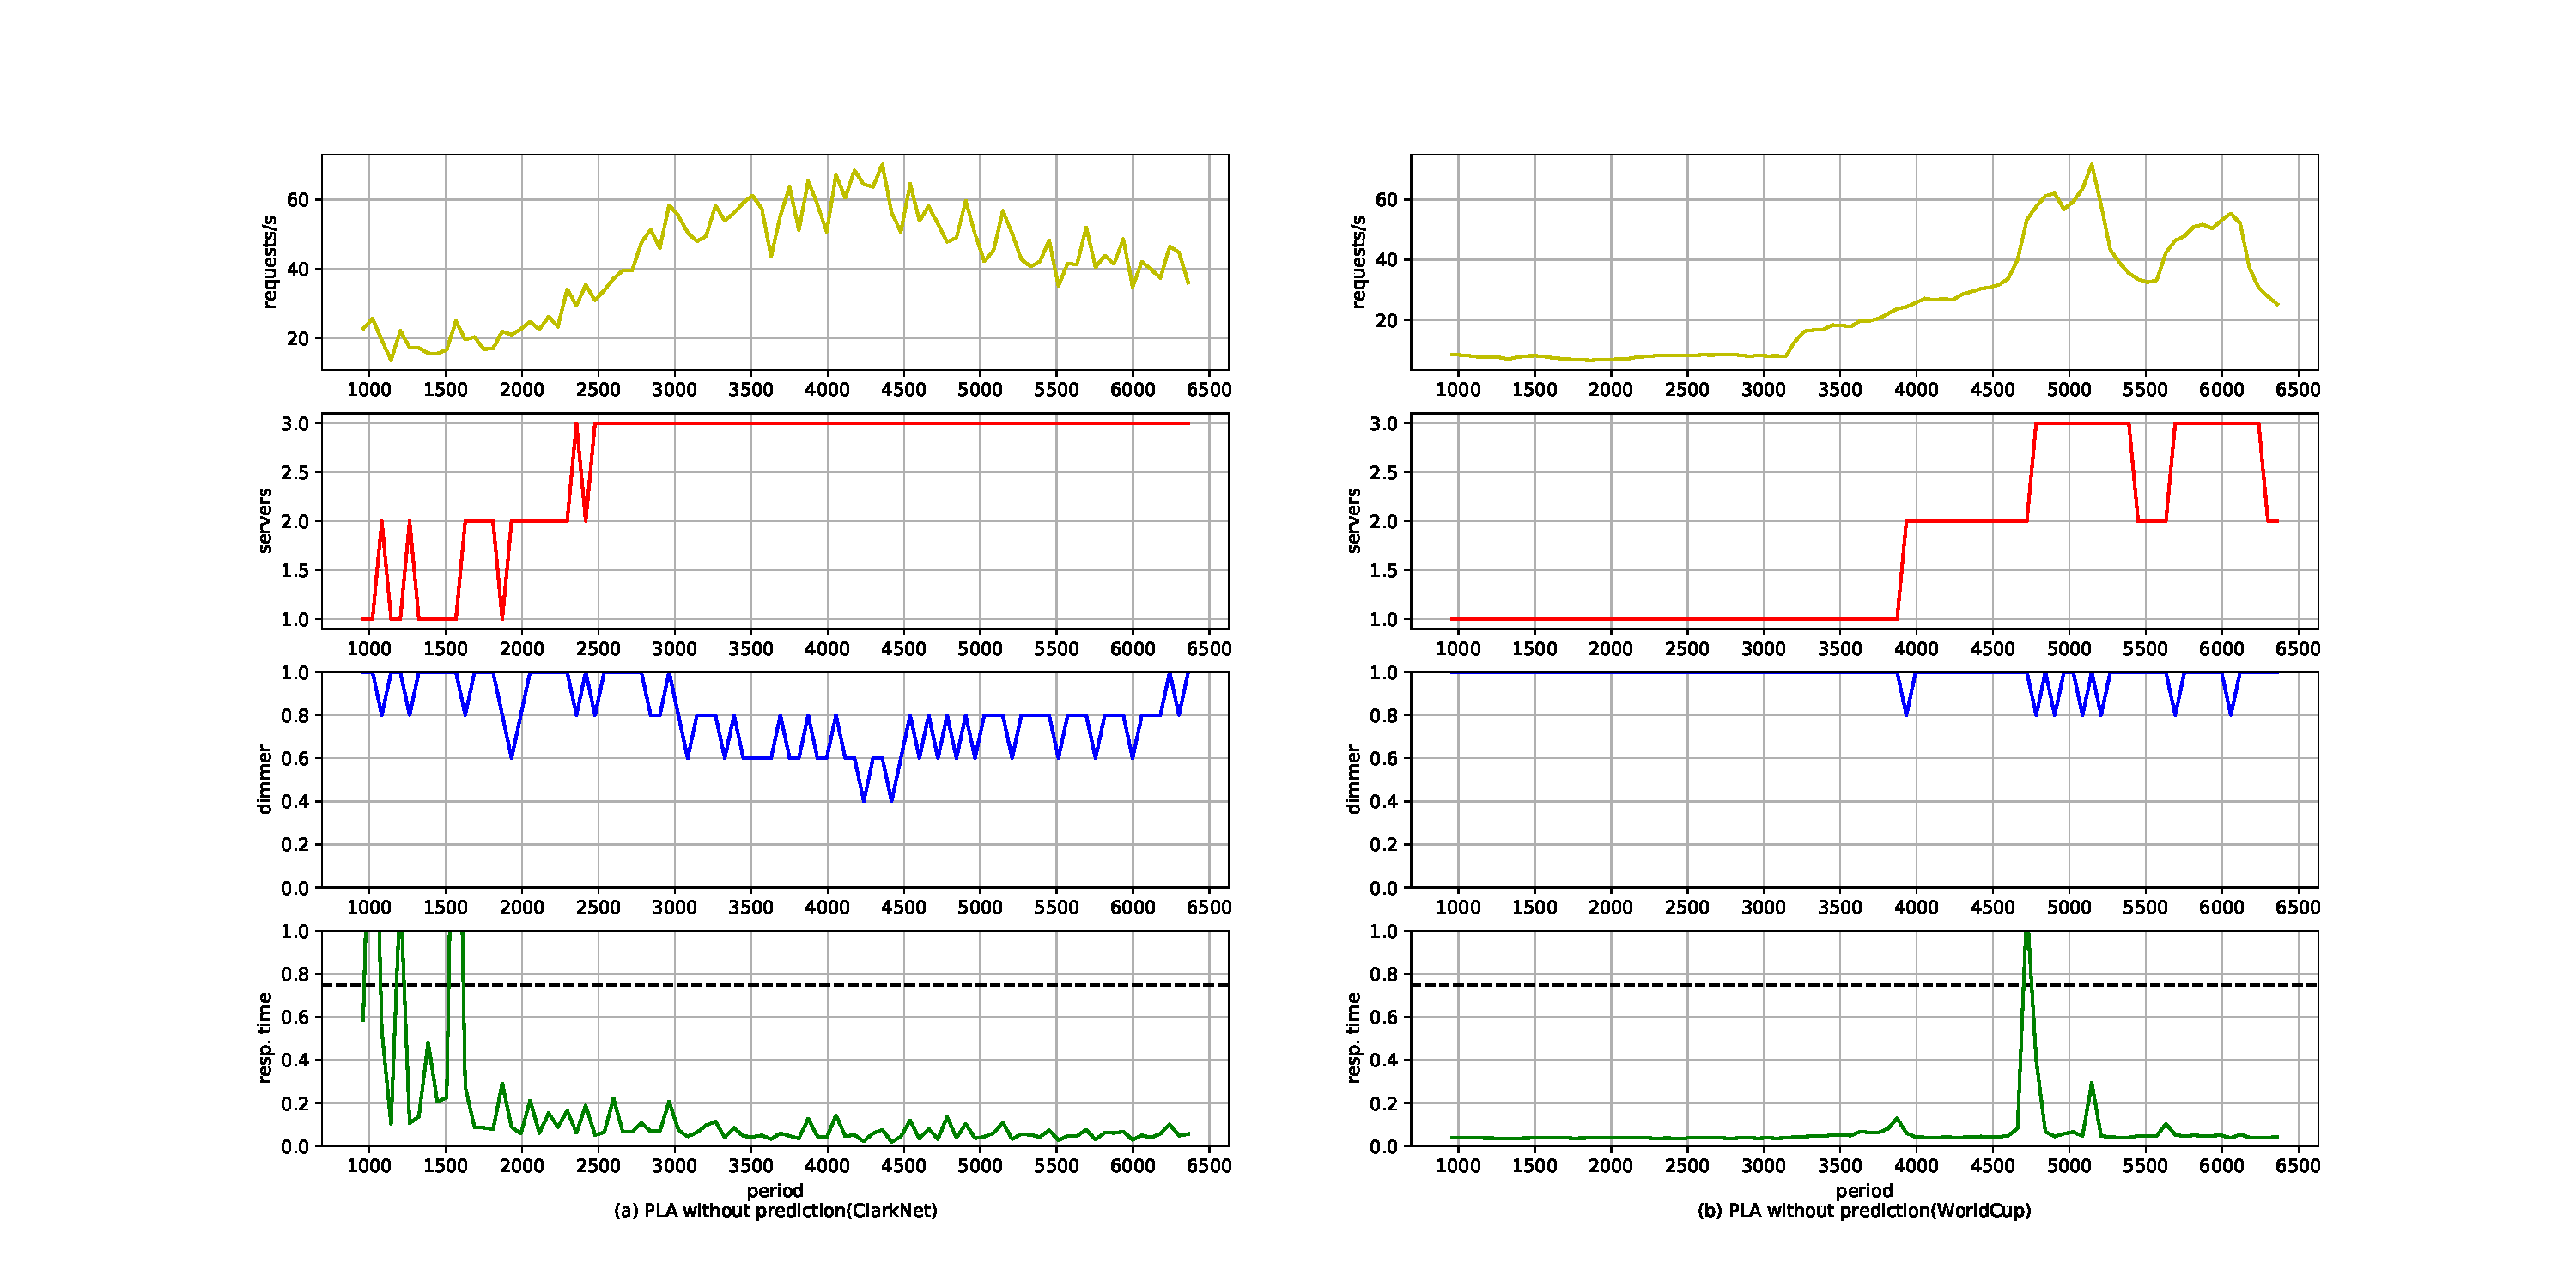
\includegraphics[width=\linewidth]{nopre}
	\caption{PLA without prediction for environment}
	\label{fig:nopre}
\end{figure}

\begin{figure}[!htp]
	\centering
	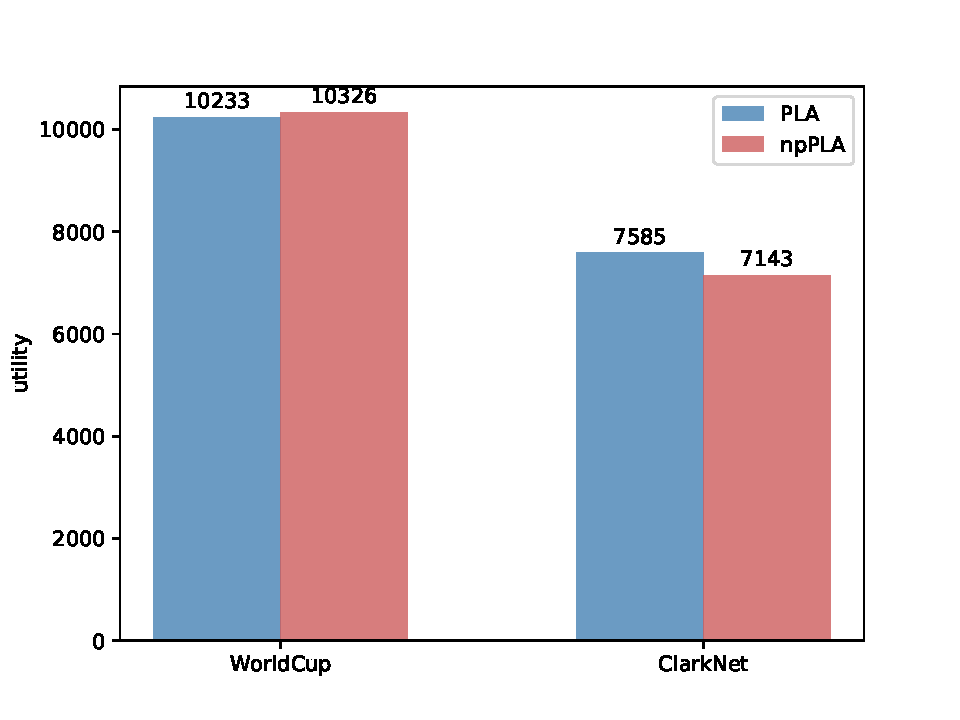
\includegraphics[width=\linewidth]{utility-np}
	\caption{Utility of PLA and npPLA}
	\label{fig:utility-np}
\end{figure}

\subsection{Linear Model \& Exponential Model}
One of the most significant differences between the PLA and CobRA is system modeling which quantize the relationship of indictors and adaptation parameters. PLA regards the managed system as white-box and pays much effots on precise modeling. For example, it use LPS queuing model to predict the average response time under specified servers and dimmer. CobRA assumes that the managed system is in vicinity of a equilibrum point despite of uncertainties~\cite{Sontag2013}. Therefore, it regards the managed system as black-box and identify system model as a linear model using sampling data in vicinity of its equilibrum point. For the highly nonlinear system, such as RUBiS which is an exponential system and sensitive to fluctuation of workload, a linear model may makes poor self-adaptation. 

In this section, we want to discuss the contributions of PLA's precise model to a good self-adaptation. We design a variant PLA named linearPLA to discuss the effectiveness of precise model. The same as CobRA, linearPLA uses a time-invariant liear model to describe the system instead of exponential LPS model. As shown in Figure ~\cite{prePLA}, if the prediction value of precise model are consistent with the measurements, precise modeling can significant improve the self-adaptation performance. 

However, the precise system model of RUBiS is a steady state approximation of LPS queue in heavy traffic~\cite{zhang2008steady} and there are significant deviations between predicted indictors and their transient measurements which is relied on feedback mechanism to offset. Figure~\ref{linearPLA} shows its adaptation process with the same two workloads and Figure~\ref{utility-l} shows the utilities of PLA with a precise model and a linear model respectively. Although linear model is more inaccurate than LPS model, they can get about the same adaptation effects because of large deviation of precise model prediction. In conclusion, if the precise system model and other predction models also have signficant model uncertainties, a linear model with a good designed feedback mechanism is a good choice to implementing self-adaptation.

\subsection{Asymmetrical Latency}
In RUBiS system, there is a certain latency when adding a server, but removing a server can be regarded to be no delay. That means there is an asymmetrical latency with the control parameter $s$.

PLA models asymmetrical latency of each tactics into the state transistion while CobRA does not  take asymmetrical latency into account. In control engineering, it will cost the same time to shown the effect of increasing or decreasing the values of control parameters, namely the adding/increase or removing/decrease adaptation tactics corresponding to a control parameter is instant or have the symmetrical latency. Therefore, CobRA forces to model the tactic delay as symmetric. for example, removing server is also considered to have the same latency distribution of booting a server. Because of CobRA's receding horizon, when the workload is decreasing and there is no need to use more servers in the horizon, considering the latency of removing server, CobRA will make the decision to reduce the server in advance and increase dimmer value to compensate the latency which may reduce the adapation performance.

In order to discuss the influence of asymmetrical latency to CobRA's adaptation performance, we change the latency of adding a server ranging from 30s to 180s. Figure~\ref{latency} shows the control result and Figure~\ref{utility-latency} shows their utilities. When latency increases to 180s, the utility of CobRA has a significant decline. We transform RUBiS system to have symmetrical latency of executing server numbers. 

We assume that the linear model of the system is obtained through system identification: 

\begin{equation}
r=k_1 *s+k_2 *d+k_3*a
\end{equation}

To translate this into a state space model, we use the state matrix $A$ to reflect the latency of adding a server. The matrixs in the state space model of (4) are:

$A={\left[\begin{array}{ccc}
	0&0&0\\
	1&0&0\\
	0&0&0\\
	\end{array}
	\right]
}$, $B={\left[\begin{array}{ccc}
	1&0\\0&0\\
	0&1\\
	\end{array}
	\right]}$,

$C={\left[\begin{array}{ccc}
	1&0&0\\
	0&0&1\\
	0&k_1&k_2\\
	\end{array}
	\right]
}$, $D={\left[\begin{array}{ccc}
	0\\
	0\\
	k_3\\
	\end{array}
	\right]
}$.

\noindent That is: 
\begin{equation}
r(k)=k_1 *s(k-2)+k_2 *d(k-1)+k_3*a(k-1)
\end{equation}

Under this model, it can be found that at time $k$, the number of servers used is the measured value at time $k-2$, namely removing servers is also modeled with a delay. When the adaptation decision is to reduce the number of servers, in order to maximize the revenue, it will remove a server ahead of time and increase dimmer to compensate for the impact of  forced removing delay. This may cause the actual response time to exceed the threshold and, if not, reduce the load fluctuations the system can withstand.

One way to modify CobRA to allow for asymmetrical latency is to use a dual model. We can design another system model to be used when removing the server, and the state matrix A is the matrix that does not reflect the delay, $A={\left[\begin{array}{ccc}
	0&0&0\\
	0&0&0\\
	0&0&0\\
	\end{array}
	\right]
}$, While optimizing the solution, the corresponding model is used when the decision of reducing the server occurs. 
However, there are many factors need to consider when using multi-model switching of CobRA, such as when and how to switch the models to ensure system states are stable. 

\subsection{Regularization}
In CobRA's cost-funtion, it has constraints on the actuation of control parameters, prefer as little change as possible according to the weight matrixs. However, PLA does not constraint on the actuations. In addition to the expected value of indicators, it is also clear that users are concerned about actuation of control parameters. Frequently actuating the control parameters will cause expensive costs or specific efforts. Consequently, CobRA takes the input signal into account. However, for our experiment, RUBiS is just able to adjust discretely and servers are only allowed to increase one at a time, the difference between PLA and CobRA is not so much serious. We can regard it as when there are more than one ways to achieve maximun utility, CobRA prefers to choose the one with less actuation of control parameters while PLA will choose at random. When there can be huge adjustments, it will make a big difference.

\section{conclusion}
Based on the work of ~\cite{moreno2017comparing}, we analyze and compare the similarities and differences between PLA and CobRA for guiding the approch selection when implementing software self-adaptation.

Gabriel et al. have validate that the two approaches can achieve similar adaptation effects. We explore the principle of this similarity. Then, we enumerate and analyze the major four differences between the two approaches. We find that the adaptation performance of PLA are high relied on feedback mechanism when there are significant devirations in model prediction and system precise modeling, leading to the similar adaptation performance of PLA without environment prediction and with linear modeling respectively. In addition, PLA can model asymmetrical latency of adding servers, while CobRA can not model it but can tolerate a certain degree of model inaccuracy. Moreover, CobRA explicitly constraits on how much the control parameters can be adjusted comparing to PLA.

In my future work, .
\bibliographystyle{ACM-Reference-Format}
\bibliography{acmart}
\end{document}
\endinput

